\section{CEGIS}
\label{sec:cegis}

Program se može sintetisati tako što se definišu njegove specifikacije i zapišu u vidu formule koja se prosledi SMT rešavaču (kao što je na primer Z3). SMT nađe valuaciju koja je zadovoljiva i to predstavlja rešenje. Problem nastaje u tome što formula koja se prosleđuje rezavaču sadrži univerzalne kvantifikatore koje usporavaju pretragu. Naime, rešavač bi u svakom slučaju pronašao rešenje za datu formulu, ali kako bi se to desilo u realnom vremenu, CEGIS (\emph{Counter-Example Guided Inductive Synthesis}) u sebi sadrži posebnu taktike za optimizaciju.

Za većinu realnih problema nije neophodno da se razmatraju svi ulazi i izlazi kako bi se došlo do programa koji radi tačno za svaki od njih. Ovako razmišljajući, problem se menja i postaje: \emph{koji je najmanji podskup ulaza koji je potrebno razmatrati da bi se sintetisao program koji zadovoljava date specifikacije?}
CEGIS tehnika upravo traga za tim minimalnim skupom. U petlji, korišćenjem SMT rešavača, on postepeno dolazi do svih mogućih implementacija željenog programa koristeći sve ulaze koji su razmatrani do tog trenutka (počinje sa 0 ulaza). U sledećoj iteraciji on razmatra dalje. Paralelno sa tim, drugim SMT rešavačem pronalazi kontra-primer koji pokazuje da poslednji sintetisani program nije rešenje. Ukoliko kontra-primer ne postoji, poslednji sintetisani prigram je rešenje. Ukoliko se prođe kroz sve iteracije i ne pronađe se rešenje, specifikacija programa nije smislena.

Jedna od mogućih implementacija se može naći na \cite{CEGISimpl}.

\subsection{Arhitektura}
\label{subsec:Arhitektura}

The general architecture of CEGIS-based synthesizers is given in \ref{fig:cegisArch} and consists of two phases, the inductive generalization and the verification oracle, which interact via a set of test vectors INPUTS that is updated incrementally. Given some specification, the inductive generalization phase tries to synthesize a candidate solution that works correctly for the current finite set of inputs.

staviti ref na ovo zbog slike: https://www.ncbi.nlm.nih.gov/pmc/articles/PMC5597726/


\begin{figure}[h!]
\begin{center}
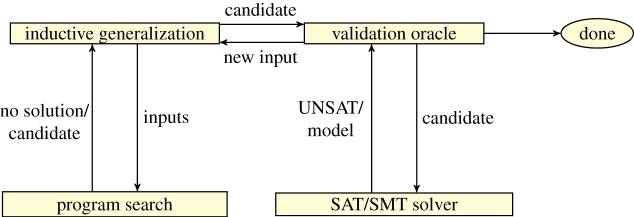
\includegraphics[scale=0.4]{resources/cegis.jpeg}
\end{center}
\caption{CEGIS petlja}
\label{fig:cegis}
\end{figure}


\subsection{Primene CEGISa}
\label{subsec:primeneCEGISa}

Ovo je jedan mogući podnaslov.
